% V-SIL.tex — V-SIL: a three-layer governed lifecycle for LLM-assisted SDR FM spectrum sensing
% Author: David Ramírez-Betancourt — Universidad Nacional de Colombia (GCPDS)
% Self-contained: no \input, no \include, inline bibliography.
\documentclass[11pt,a4paper]{article}
\usepackage[margin=2.5cm]{geometry}
\usepackage[utf8]{inputenc}
\usepackage[T1]{fontenc}
\usepackage{amsmath}
\usepackage{amssymb}
\usepackage{booktabs}
\usepackage{array}
\usepackage{enumitem}
\usepackage{xcolor}
\usepackage{tikz}
\usetikzlibrary{positioning, shapes.geometric, arrows.meta, calc, fit, backgrounds}
\usepackage{hyperref}
\usepackage[noabbrev,capitalise]{cleveref}

% ---------------------------------------------------------------------------
% Color definitions (per PLAN)
% ---------------------------------------------------------------------------
\definecolor{coral}{HTML}{f87171}
\definecolor{vblue}{HTML}{3b82f6}
\definecolor{vteal}{HTML}{14b8a6}
\definecolor{vred}{HTML}{ef4444}
\definecolor{amber}{HTML}{f59e0b}
\definecolor{violet}{HTML}{8b5cf6}
\definecolor{vgrey}{HTML}{6b7280}

\hypersetup{
  colorlinks=true,
  linkcolor=vblue!70!black,
  citecolor=vteal!70!black,
  urlcolor=vblue!70!black
}

\setlist[itemize]{leftmargin=1.4em, topsep=0.35em, itemsep=0.15em}
\setlist[enumerate]{leftmargin=1.7em, topsep=0.35em, itemsep=0.15em}

\newcommand{\verified}{\emph{verified}}
\newcommand{\validated}{\emph{validated}}

\title{\textbf{V-SIL}: A Three-Layer Governed Lifecycle for\\[4pt]
LLM-Assisted Development of SDR-Based FM Spectrum-Sensing Systems}
\author{David Ramírez-Betancourt \\
Universidad Nacional de Colombia --- GCPDS}
\date{October 2026}

\begin{document}
\maketitle
\thispagestyle{empty}

\begin{abstract}
\noindent
Spectrum-sensing systems built on software-defined radio (SDR) must produce measurements that are
traceable, reproducible, and defensible against regulatory criteria. When large language models
(LLMs) are used to assist the engineering of such systems, the classical verification problem
becomes harder: the generator is probabilistic, and its behaviour can drift without any change to
the source tree, silently invalidating the evidence that once justified a prototype. This paper
presents \textbf{V-SIL}, a three-layer governed lifecycle that integrates conceptual validation
(the zz\_Workflow prototype-development engine), continuous software development
(CI with Software-in-the-Loop), and post-development operations (the Production Pipeline, PCG)
into a single, auditable pipeline for SDR FM broadcast compliance monitoring. Layer~1 defines and
validates the concept through context-bounded stages, human readiness gates, and six governing
artefacts. Layer~2 makes the V-model's right arm continuous: the same test levels run on every
commit, merge, and nightly build against a Mock HAL fed by synthetic I/Q, with deterministic
acceptance gates. Layer~3 governs the deployed array through a circular five-stage production
pipeline, a versioned promotion and rollback gate, capability-class maturation, GUM uncertainty
propagation, and append-only evidence archiving. The coupling between layers is clean because
each layer's terminal output is the next layer's input. Claims stay honest by construction:
systems are \emph{verified} at software-in-the-loop and \emph{validated} only on real hardware,
and the model never approves its own work.
\end{abstract}

\tableofcontents
\newpage

% ===========================================================================
\section{Introduction}
\label{sec:intro}

Radio-spectrum monitoring for broadcast compliance is a measurement problem before it is a
software problem. An SDR-based sensor sweeps the FM broadcast band, estimates power spectral
density, and decides whether a channel is occupied by a licensed emitter, by an interferer, or by
noise. Every one of those decisions can carry regulatory consequences, so the chain from raw I/Q
samples to an occupancy declaration must be traceable: the configuration, the software version,
the calibration state, and the uncertainty of the measurement all have to be reconstructable
after the fact. At the same time, the engineering effort behind such a sensor is increasingly
\emph{LLM-assisted}: language models draft code, DSP block configurations, test cases, and even
regulatory analyses under human supervision.

This assistance introduces a failure mode that classical software engineering did not have to
treat as first-class. An LLM is probabilistic, not deterministic: outputs vary even at nominal
zero temperature, because the inference stack itself contributes a background temperature
\cite{pith2026}. Agent reliability decays roughly geometrically with the number of sequential
steps \cite{mittal2026}, and benchmark incentives reward confident guessing over abstention, so
models are trained to hallucinate \cite{kalai2026}. The practical consequence for a verification
pipeline is severe: once a prototype exists, \textbf{every later change to code, prompt, model,
or context document can silently invalidate the evidence that justified it}, even when the
source tree is untouched \cite{mittal2026,kalai2026}. A verification strategy that assumes a
fixed generator is therefore built on sand.

Two structural responses are already known from the systems-engineering literature. First,
\emph{structure beats instructions}: reliability gains come mainly from typed interfaces, gates,
retries, and explicit state rather than from longer prompts \cite{nerd2026}, and context
engineering---what the model sees at each step, and nothing more---outranks prompt engineering
\cite{anthropic2026}. Second, \emph{an external oracle must decide}: the component that generates
work must never be the component that approves it \cite{judge2026}, because optimization pressure
readily exploits evaluator weaknesses in a self-evaluating system. Empirically the gap is real:
roughly 83\% of autonomous-research agents publish code, but only 38\% provide reproducible
artifacts \cite{verifgap2026}.

\textbf{Thesis.} V-SIL integrates three already-developed bodies of methodology into a single
governed lifecycle for the SDR FM sensor:

\begin{itemize}
  \item \textbf{Layer 1 --- Conceptual Validation} (source: the zz\_Workflow
    prototype-development engine): four context-bounded stages (Ctx 00--03) that define and
    validate \emph{what to build}, protected by human readiness gates and closed by a
    \emph{Verified Prototype + Evidence}.
  \item \textbf{Layer 2 --- Software Development} (source: CI+SIL): continuous integration with
    software-in-the-loop, which keeps the V-model's four test levels but makes the right arm
    continuous, triggering on every code, prompt, model, or context change.
  \item \textbf{Layer 3 --- Post-Development Operations} (source: the Production Pipeline, PCG):
    a circular five-stage pipeline that governs the deployed array, its calibration, its
    uncertainty, and its audit-ready evidence.
\end{itemize}

The layers are not alternatives; they are complementary stages of one lifecycle. Layer~1
validates the concept and the design---not the software. Layer~2 implements and continuously
verifies the software. Layer~3 operates the system in production under metrological and
regulatory governance. Detail is deferred to \cref{sec:layer1,sec:layer2,sec:layer3};
\cref{sec:overview} gives the integrated picture.

% ===========================================================================
\section{V-SIL Overview}
\label{sec:overview}

\cref{fig:vsil} shows the V-SIL lifecycle as a whole. The upper part is the classical V shape:
a descending left arm that defines the system, an ascending right arm that tests it, and a
valley where implementation happens. Each left-hand level \emph{defines the tests} for the
right-hand level that mirrors it (dashed links). V-SIL re-reads the right arm as continuous
software-in-the-loop: the unit, integration, and system levels run on every commit, merge, and
nightly build respectively, against a Mock HAL fed by synthetic I/Q---no live RF is required.
Only the apex, acceptance testing, remains at hardware-in-the-loop with the real device: it is
the one level CI does not absorb, and the honest boundary of the whole verification apparatus.
Below the V, the PCG pipeline (Layer~3) governs the deployed system as a closed loop of five
stages, from the development sandbox to metrological guardrails and back.

\begin{figure}[htbp]
\centering
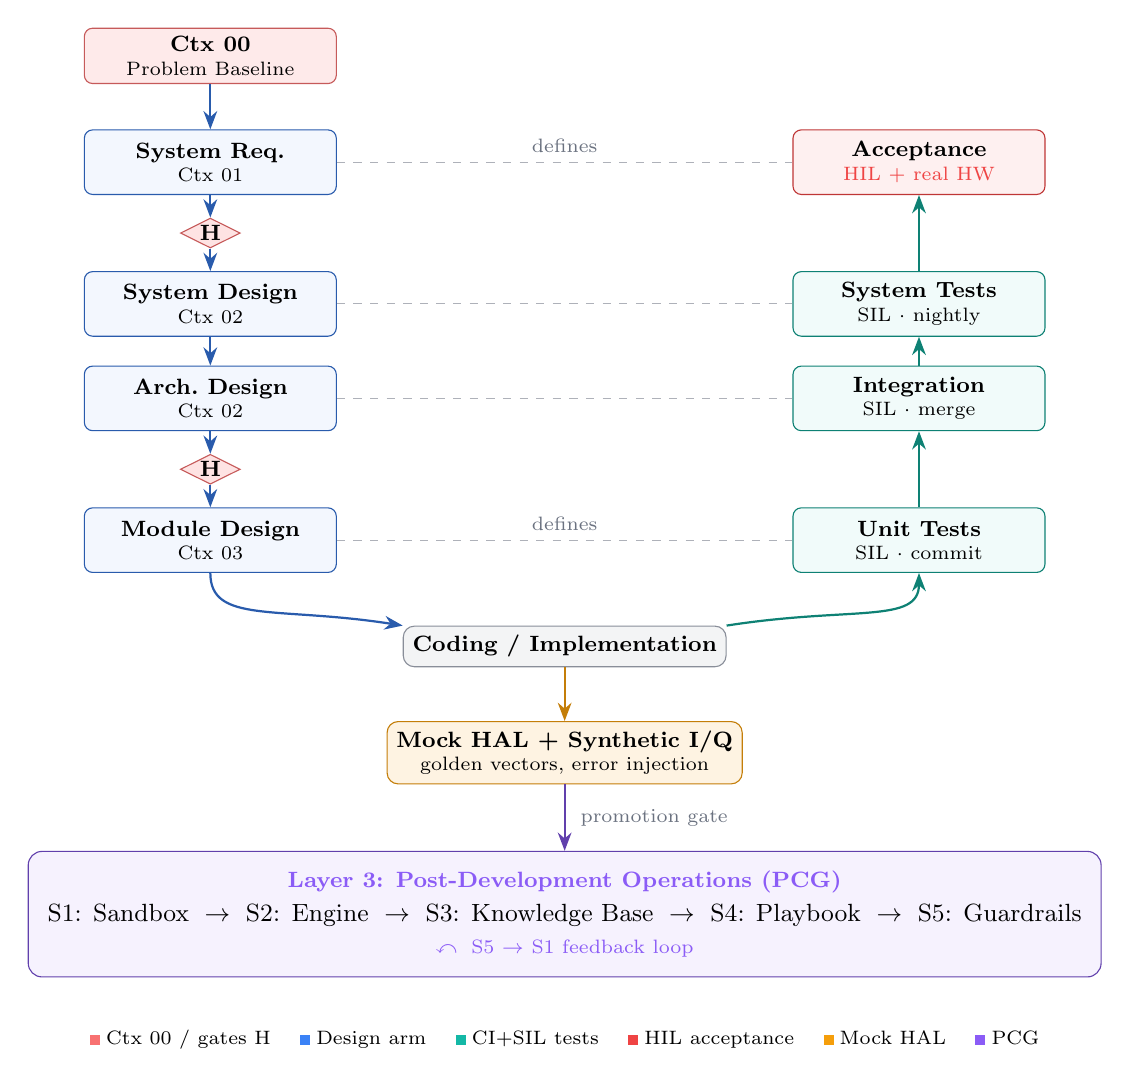
\begin{tikzpicture}[
  font=\footnotesize,
  >={Stealth[length=2.4mm]},
  armL/.style={draw=vblue!70!black, fill=vblue!6, rounded corners=3pt,
               align=center, minimum width=3.2cm, minimum height=0.82cm, inner sep=3pt},
  armR/.style={draw=vteal!70!black, fill=vteal!6, rounded corners=3pt,
               align=center, minimum width=3.2cm, minimum height=0.82cm, inner sep=3pt},
  hil/.style={armR, draw=vred!80!black, fill=vred!8},
  gate/.style={draw=coral!80!black, fill=coral!20, diamond, aspect=2,
               inner sep=0.5pt, font=\footnotesize\bfseries},
  fL/.style={draw=vblue!70!black, thick, -{Stealth}},
  fR/.style={draw=vteal!70!black, thick, -{Stealth}},
  def/.style={draw=vgrey!55, dashed, thin}
]

% ---- Left arm (design, descending) ----
\node[draw=coral!80!black, fill=coral!15, rounded corners=3pt, align=center,
      minimum width=3.2cm, inner sep=3pt] (ctx00) at (-4.5,7.4)
      {\textbf{Ctx 00}\\[-1pt]{\scriptsize Problem Baseline}};

\node[armL] (l1L) at (-4.5,6.05) {\textbf{System Req.}\\[-1pt]{\scriptsize Ctx 01}};
\node[gate] (g1)  at (-4.5,5.15) {H};
\node[armL] (l2L) at (-4.5,4.25) {\textbf{System Design}\\[-1pt]{\scriptsize Ctx 02}};
\node[armL] (l3L) at (-4.5,3.05) {\textbf{Arch.\ Design}\\[-1pt]{\scriptsize Ctx 02}};
\node[gate] (g2)  at (-4.5,2.15) {H};
\node[armL] (l4L) at (-4.5,1.25) {\textbf{Module Design}\\[-1pt]{\scriptsize Ctx 03}};

\draw[fL] (ctx00.south) -- (l1L.north);
\draw[fL] (l1L.south)   -- (g1.north);
\draw[fL] (g1.south)    -- (l2L.north);
\draw[fL] (l2L.south)   -- (l3L.north);
\draw[fL] (l3L.south)   -- (g2.north);
\draw[fL] (g2.south)    -- (l4L.north);

% ---- Right arm (test, ascending) ----
\node[hil]  (l1R) at (4.5,6.05) {\textbf{Acceptance}\\[-1pt]
  {\scriptsize\color{vred}HIL + real HW}};
\node[armR] (l2R) at (4.5,4.25) {\textbf{System Tests}\\[-1pt]
  {\scriptsize SIL $\cdot$ nightly}};
\node[armR] (l3R) at (4.5,3.05) {\textbf{Integration}\\[-1pt]
  {\scriptsize SIL $\cdot$ merge}};
\node[armR] (l4R) at (4.5,1.25) {\textbf{Unit Tests}\\[-1pt]
  {\scriptsize SIL $\cdot$ commit}};

% Ascending arrows: bottom-up, .north to .south
\draw[fR] (l4R.north) -- (l3R.south);
\draw[fR] (l3R.north) -- (l2R.south);
\draw[fR] (l2R.north) -- (l1R.south);

% ---- Dashed "defines" links (node edge to node edge) ----
\draw[def] (l1L.east) -- (l1R.west)
  node[midway, above, font=\scriptsize, text=vgrey] {defines};
\draw[def] (l2L.east) -- (l2R.west);
\draw[def] (l3L.east) -- (l3R.west);
\draw[def] (l4L.east) -- (l4R.west)
  node[midway, above, font=\scriptsize, text=vgrey] {defines};

% ---- Valley ----
\node[draw=vgrey!80, fill=vgrey!8, rounded corners=4pt, align=center,
      minimum width=3.4cm] (valley) at (0,-0.1)
      {\textbf{Coding / Implementation}};

% Smooth V curves into the valley
\draw[fL] (l4L.south) .. controls ++(0,-0.65) and ++(-1.6,0.25) .. (valley.north west);
\draw[fR] (valley.north east) .. controls ++(1.6,0.25) and ++(0,-0.65) .. (l4R.south);

% ---- Mock HAL ----
\node[draw=amber!80!black, fill=amber!12, rounded corners=4pt, align=center,
      minimum width=3.4cm] (mock) at (0,-1.45)
      {\textbf{Mock HAL + Synthetic I/Q}\\[-1pt]
       {\scriptsize golden vectors, error injection}};
\draw[draw=amber!80!black, thick, -{Stealth}] (valley.south) -- (mock.north);

% ---- PCG band (Layer 3) ----
\node[draw=violet!70!black, fill=violet!8, rounded corners=5pt, align=center,
      minimum width=11.5cm, inner sep=7pt] (pcg) at (0,-3.5)
      {\textbf{\color{violet}Layer 3: Post-Development Operations (PCG)}\\[3pt]
       {\small S1: Sandbox $\;\to\;$ S2: Engine $\;\to\;$ S3: Knowledge Base
       $\;\to\;$ S4: Playbook $\;\to\;$ S5: Guardrails}\\[2pt]
       {\scriptsize\color{violet}$\curvearrowleft$\; S5 $\to$ S1 feedback loop}};

\draw[draw=violet!70!black, thick, -{Stealth}] (mock.south) -- (pcg.north)
  node[midway, right=2pt, font=\scriptsize, text=vgrey] {promotion gate};

% ---- Legend ----
\node[anchor=north, font=\scriptsize, align=center] at (0,-4.85) {%
  \textcolor{coral}{\rule{0.45em}{0.45em}}\;Ctx 00 / gates H \quad
  \textcolor{vblue}{\rule{0.45em}{0.45em}}\;Design arm \quad
  \textcolor{vteal}{\rule{0.45em}{0.45em}}\;CI+SIL tests \quad
  \textcolor{vred}{\rule{0.45em}{0.45em}}\;HIL acceptance \quad
  \textcolor{amber}{\rule{0.45em}{0.45em}}\;Mock HAL \quad
  \textcolor{violet}{\rule{0.45em}{0.45em}}\;PCG};

\end{tikzpicture}
\caption{\textbf{V-SIL lifecycle.} A descending left arm (blue) defines the system; an ascending
right arm (teal) tests it continuously as software-in-the-loop (SIL) on commit, merge, and
nightly cadence, against a Mock HAL fed by synthetic I/Q (amber). Gates~H (coral) are human
readiness gates; acceptance (red) stays at hardware-in-the-loop with real hardware---the apex of
the V and the boundary of verification. Below the V, the PCG pipeline (violet) governs the
deployed array as a closed five-stage loop from sandbox to guardrails and back.}
\label{fig:vsil}
\end{figure}

\cref{tab:layers} summarises the three layers and the contract between them: each layer's
terminal output is the next layer's input, and each layer names the environment in which its
claims were produced.

\begin{table}[htbp]
\centering
\caption{The three layers of V-SIL and their terminal outputs.}
\label{tab:layers}
\small
\begin{tabular}{@{}clllp{4.2cm}@{}}
\toprule
\textbf{\#} & \textbf{Name} & \textbf{Source} & \textbf{Purpose} & \textbf{Terminal output} \\
\midrule
1 & Conceptual Validation & zz\_Workflow & Define and validate what to build & Verified Prototype + Evidence \\
2 & Software Development & CI+SIL & Implement and continuously verify & Regression-passing build \\
3 & Post-Development Ops & PCG & Govern the deployed system & Audit-ready evidence archive \\
\bottomrule
\end{tabular}
\end{table}

\subsection{Governing principles}
\label{sec:principles}

Four principles govern every layer. They are stated once here and enforced everywhere.

\begin{enumerate}[label=\textbf{P\arabic*.}]
  \item \textbf{HITL is an authorization barrier; HIL is a validation barrier.}
    Human-in-the-loop (HITL) means a person approves consequential actions---every readiness
    gate, every production promotion, every anomalous regulatory classification.
    Hardware-in-the-loop (HIL) means the control software is exercised against real hardware.
    The two are distinct barriers and neither substitutes for the other \cite{opalrt2026}.
  \item \textbf{Oracle $\neq$ generator --- the model never approves its own work.}
    The LLM drafts within a stage; acceptance is decided by an external, pre-declared criterion.
    When the same component proposes and evaluates, optimization pressure exploits evaluator
    weaknesses \cite{judge2026}.
  \item \textbf{Mechanical rejection beats LLM approval, never the reverse.}
    A schema violation, a failed test, or a threshold exceedance rejects work mechanically.
    Human judgment is a fallback and an escalation path, not a default approval mechanism.
  \item \textbf{\Verified{} $\neq$ \validated{} --- claims name the environment.}
    ``Verified'' means conformance to pre-declared criteria on recorded measurements in a given
    environment; ``validated'' means fitness for the monitoring objective in the field, on real
    hardware \cite{sheridan2026b}. A system verified in simulation is not thereby validated;
    the claim must name the environment in which the evidence was produced.
\end{enumerate}

% ===========================================================================
\section{Layer 1: Conceptual Validation Engine}
\label{sec:layer1}

\textbf{Source: the zz\_Workflow prototype-development engine.} Layer~1 is an LLM-assisted
workflow for building the SDR-based FM spectrum-sensing sensor. Development proceeds through
four stages, Ctx 00 through Ctx 03. Each stage is bounded by a context package---the content and
rules the model works from at that stage---and ends in a named output. Two of the four stage
transitions (Ctx 01$\rightarrow$02 and Ctx 02$\rightarrow$03) are protected by an explicit
readiness gate; the Ctx 00 output freezes the project scope, and the Ctx 03 output is checked
against acceptance criteria in the build and verification phase. At every transition, whether or
not a gate diamond is drawn, the human reviewer decides whether to proceed: the model drafts
within a stage but never approves its own output. Acceptance is decided by pre-declared criteria
applied to recorded measurements, never by model judgement.

\textbf{This layer validates the concept and the design, not the software.} Its terminal output,
\emph{Verified Prototype + Evidence}, is verification of a build against a frozen contract; it is
not field validation, and V-SIL never presents it as such.

\subsection{Ctx 00 --- Project Definition}
\label{sec:ctx00}

Ctx 00 establishes what the project is for, before any requirement or architecture exists:
project purpose and monitoring objective; intended users and operational environment; system
boundary and declared scope; and the authoritative technical and regulatory sources the whole
project will rely on. The output is the \textbf{Problem Baseline + Frozen Project Scope}. The
problem baseline is the agreed, stable definition of the problem the project is intended to
solve. Because the scope is frozen at this point, it can only be reopened through route R0 as a
controlled change---a deliberate design decision that prevents scope drift from laundering
itself as a requirement change.

\subsection{Ctx 01 --- Requirements and Constraints}
\label{sec:ctx01}

Ctx 01 turns the baseline into engineering obligations: product and system requirements
(functional and non-functional); regulatory, technical, and data-handling constraints; HackRF
capability boundaries and the target compute platform; measurable acceptance criteria; and
requirement identifiers with traceability. The output is the \textbf{Versioned Requirements
Baseline}. Two properties matter for everything downstream. First, acceptance criteria are
\emph{measurable}---they will later drive the deterministic acceptance gate of Layer~2, so an
unmeasurable criterion is not a criterion. Second, requirement identifiers exist from this point
on, so any downstream failure can be routed to the requirement that failed rather than to a
vague notion of ``the spec''.

\subsection{Gate H (Ctx 01 $\rightarrow$ 02)}
\label{sec:gate-h1}

The first readiness gate asks: \emph{Requirements complete, bounded, and verifiable?} A
\textbf{YES} admits the stage to Ctx 02; a \textbf{NO} returns the work to Ctx 01 for revision.
The gate is decided by the human reviewer, on the recorded artefacts of Ctx 01.

\subsection{Ctx 02 --- Architecture and Design Resolution}
\label{sec:ctx02}

Ctx 02 resolves the design space: candidate DSP and classification architectures; alternative
implementation pathways; hardware/software partitioning; the component dependency graph; trade
studies and design decisions; and the selection rationale. The output is the \textbf{Selected
Architecture + Implementation Plan}. The stage is explicitly multi-hypothesis: Pathway~1 through
Pathway~n are carried into an architecture trade study, and the selection is justified in writing.
This is the only place in the lifecycle where alternatives are compared; from Ctx 03 onward the
chosen architecture is contract, and changes go through defect routing rather than reconsideration.

\subsection{Gate H (Ctx 02 $\rightarrow$ 03)}
\label{sec:gate-h2}

The second readiness gate asks: \emph{All implementation-critical design choices resolved?}
\textbf{YES} admits the stage to Ctx 03; \textbf{NO} returns it to Ctx 02 for resolution. Its
purpose is to stop implementation from absorbing design decisions that were never made---the
most common way an implementation plan quietly becomes an architecture.

\subsection{Ctx 03 --- Executable Implementation Contract}
\label{sec:ctx03}

Ctx 03 is the only stage that looks like software engineering, and it produces a contract, not
code: software component contracts; the SDR acquisition and configuration contract; DSP and
classification algorithms with their processing sequence; interfaces and versioned data schemas;
configuration parameters and units; error and state behaviour (dropped samples, receiver
saturation, local-oscillator tuning delay); and the unit, integration, and acceptance tests. The
output is the \textbf{Executable Prototype Build Package}. The SDR instantiation is concrete: a
hardware sweep (for example via \texttt{hack\_rf\_sweep}), FFT and power spectral density
estimation, and classification, with declared fallback behaviour for each non-ideality. Layer~2
consumes this package as an executable specification (\cref{sec:l1-l2}).

\subsection{Build, verification, and defect routing}
\label{sec:routing}

The build package is built and integrated (configure HackRF $\rightarrow$ acquire I/Q $\rightarrow$
process DSP and classification $\rightarrow$ generate measurements $\rightarrow$ store, transport,
visualize), exercised in a \textbf{reproducible verification run} (execute the declared test
configuration, measure outputs against acceptance criteria, record logs, configurations,
measurements, and test evidence), and assembled into a \textbf{Verification Evidence Package}:
requirement ID $\rightarrow$ test ID $\rightarrow$ result; configuration and software versions;
RF measurement evidence; observed deviations and uncertainty; and a reproducible execution
record. The final gate asks: \emph{All mandatory acceptance criteria satisfied?}

\begin{itemize}
  \item \textbf{YES} $\rightarrow$ \textbf{Verified SDR Prototype + Traceable Verification
    Evidence} $\rightarrow$ \textbf{Critical Reflection}: validation against the monitoring
    objective, residual limitations, lessons learned, next-version requirements, and research
    questions.
  \item \textbf{NO} $\rightarrow$ \textbf{Failure Classification}: the defect is classified by
    root cause and routed to the stage responsible for it (\cref{tab:routing}).
\end{itemize}

\begin{table}[htbp]
\centering
\caption{R0--R3 defect routing: every failure returns to the stage that owns its root cause.}
\label{tab:routing}
\small
\begin{tabular}{@{}clp{7.4cm}@{}}
\toprule
\textbf{Route} & \textbf{Returns to} & \textbf{Root-cause class} \\
\midrule
R0 & Ctx 00 & Problem/scope defect --- reopened only through change control \\
R1 & Ctx 01 & Requirement defect (missing, wrong, or unverifiable criterion) \\
R2 & Ctx 02 & Design/architecture defect \\
R3 & Ctx 03 & Implementation defect \\
\bottomrule
\end{tabular}
\end{table}

The routing discipline is what makes defect data actionable: a recurring R1 pattern is evidence
that the requirements process is weak, not that the code is unlucky. Layer~2 reuses the same
routing for CI failures (\cref{sec:layer2}), and Layer~3's Stage~5 feedback loop is its
operational counterpart (\cref{sec:layer3}).

\subsection{The six governing artefacts}
\label{sec:artefacts}

Six artefacts govern how the model is used within the engine
(\cref{tab:artefacts}). Each states why the artefact is needed, its role in the workflow, and how
it is instantiated for the SDR FM sensor.

\begin{table}[htbp]
\centering
\caption{The six governing artefacts of Layer~1 and where each applies.}
\label{tab:artefacts}
\small
\setlength{\tabcolsep}{5pt}
\begin{tabular}{@{}clp{4.4cm}p{6.2cm}@{}}
\toprule
\textbf{\#} & \textbf{Artefact} & \textbf{Where it applies} & \textbf{SDR instantiation} \\
\midrule
1 & System \& Prompt Architecture Map & Ctx 00--03 (concrete at Ctx 02--03); failure routing & Ctx 03 contract fixes the chain (sweep $\rightarrow$ FFT/PSD $\rightarrow$ classification) and fallbacks for drops, saturation, tuning delay \\
2 & Context \& Retrieval Specs & Sources declared in Ctx 00; populates every Ctx package & ITU and national allocation databases, modulation standards, HackRF capability/calibration data, local noise-floor baselines \\
3 & Eval \& Benchmarking Suites & Acceptance criteria (Ctx 01); tests (Ctx 03); verification run; regression after any model, prompt, or Ctx change & Golden synthetic/controlled-source I/Q at known SNR; metrics: $P_d$, $P_{fa}$, accuracy under multipath and phase noise, inference latency \\
4 & Safety \& Guardrail Design Rules & Constraints (Ctx 01); error/state behaviour (Ctx 03); all gates & Below an SNR threshold the sensor reports ``Uncertain'' rather than ``Free''; behaviour tested in verification \\
5 & AI Feedback \& Telemetry Specs & Evidence package; failure classification (R0--R3) & Deviations (missed detections, false alarms, re-tuning) logged with configuration and software versions, linked to failure class \\
6 & Data Privacy, Governance \& Compliance Specs & System boundary (Ctx 00); constraints (Ctx 01); anything leaving the local environment & Sensor constrained to un-demodulated features (PSD, spectrograms); retained I/Q is synthetic or locally governed \\
\bottomrule
\end{tabular}
\end{table}

Two artefacts deserve emphasis because they carry the coupling to the other layers. \textbf{Artefact~3}
(eval and benchmarking suites) exists because conventional unit testing cannot detect semantic
drift, hallucination, or regression when the model, a prompt, or a context package changes; its
golden test vectors are synthetic or controlled-source I/Q samples at known signal-to-noise
ratios, and it already serves double duty as the acceptance suite defined in Ctx 01. In
Layer~2, this artefact \emph{is} the CI regression harness---the coupling requires no new
concept, only automation. \textbf{Artefact~6} is the sharpest constraint on an LLM-assisted
pipeline: specifications, code, and derived metrics may be shared with third-party model
providers, but captured I/Q and any demodulated content stay local; if any stage demodulates,
audio and payload data are redacted on the device before storage or transmission so that private
communications are never recorded.

\subsection{The role of the model in Layer 1}
\label{sec:llmrole}

The LLM's role is bounded by construction. It drafts within a stage, from the context package
that stage declares; it never approves its own output, because every gate decision is reserved
for the human reviewer. Artefact~4 enforces that no model output enters a baseline without a
traceable source or test, and marks unsupported statements as unverified. Artefact~5 turns
reviewer behaviour---edits, rejected drafts, retry counts, gate outcomes, defect classes---into
an operational dataset for refining prompts and context packages, so that recurring failure
classes point to the Ctx package that needs revision. What emerges is a discipline that does not
trust the model's self-assessment: self-reported correctness is weak evidence when benchmarks
reward hallucination \cite{kalai2026}, so the workflow substitutes recorded measurements under
pre-declared criteria.

% ===========================================================================
\section{Layer 2: Software Development (CI+SIL)}
\label{sec:layer2}

\textbf{Source: CI+SIL}. Layer~1 produces a contract and a prototype; it does not keep them
verified. Once a prototype exists, every later change to code, prompt, model, or context document
can invalidate the evidence that justified it. Layer~2 is the answer: continuous integration with
software-in-the-loop, which is best understood not as a rival to the V-model but as \emph{the
V-model's right arm made continuous} \cite{sheridan2026a}.

\subsection{The V-model right arm made continuous}
\label{sec:continuous}

The classic V-model pairs a descending design/verification arm with an ascending
testing/validation arm \cite{qmsdoc2026,sheridan2026b}. Each left-hand level defines the tests
for the right-hand level that mirrors it: requirements $\leftrightarrow$ acceptance, system
design $\leftrightarrow$ system test, architecture $\leftrightarrow$ integration, module design
$\leftrightarrow$ unit test. The model is strong on traceability and on separating verification
from validation, but in its classic form the entire right arm is a single, late pass: tests run
once, after the full descent and ascent, and the oracle arrives at the end.

CI+SIL keeps the same four test levels and changes \emph{when} and \emph{against what} they run
(\cref{fig:vsil}, right arm). Instead of one late pass, the levels execute automatically and
continuously against a software-modelled plant---the SIL rung of the MIL$\rightarrow$SIL
$\rightarrow$PIL$\rightarrow$HIL ladder \cite{opalrt2026,sheridan2026a}:

\begin{itemize}
  \item \textbf{Unit} (pure logic) runs \emph{on every commit};
  \item \textbf{Integration} (SIL) runs \emph{on every merge};
  \item \textbf{System} (extended SIL) runs \emph{nightly};
  \item \textbf{Acceptance} stays at the apex as \textbf{HIL + real hardware}---the one level
    CI+SIL does not absorb, and the shared downstream gap (\cref{sec:gaps}).
\end{itemize}

\subsection{Mock HAL and synthetic I/Q}
\label{sec:mockhal}

To run the lower arm without RF, CI+SIL adds a thin substitution layer (\cref{fig:vsil},
amber). A \textbf{HAL} abstracts the device behind an interface; a \textbf{Mock HAL} of driver
stubs implements that interface in software; and \textbf{synthetic data}---golden I/Q vectors at
known SNR and injected error cases---feeds the mock. Purchased hardware sits behind the
\emph{same} HAL, so the swap from mock to real device is transparent to the code under test:
the same code path that runs in CI runs on the bench, which is what makes SIL evidence
transferable rather than merely available. The substitution is honest about its limits. It
verifies logic, DSP behaviour against known vectors, and regression stability; it cannot
validate RF front-end behaviour, and V-SIL never claims it does.

\subsection{Artefact 3 as the regression harness}
\label{sec:artefact3}

The coupling to Layer~1 costs no new concept. The evaluation and benchmarking suites that
zz\_Workflow already requires (Artefact~3) \emph{are} a CI harness: they contain golden datasets,
performance metrics (latency versus accuracy), and evaluation metrics (factual accuracy against
sources, schema and traceability checks, detection performance against known I/Q). Coupling CI
to them means the suites run automatically instead of manually, and the evidence produced at the
end of Layer~1 seeds the regression baseline. The Ctx 03 contract, together with the code, serves
as an executable specification under version control.

\subsection{Triggers: not just commits}
\label{sec:triggers}

For a probabilistic generator, a code commit is the least interesting trigger. The CI pipeline
fires on four classes of change:

\begin{enumerate}
  \item \textbf{Code change} --- the classical trigger;
  \item \textbf{Prompt change} --- rewording alters model behaviour without touching code;
  \item \textbf{Model change} --- upgrading or swapping the model shifts the generator itself;
  \item \textbf{Context change} --- editing a Ctx package or a retrieval corpus changes what the
    model sees, and context engineering outranks prompt engineering \cite{anthropic2026}.
\end{enumerate}

Each trigger replays golden I/Q through the SIL pipeline and compares the result---$P_d$,
$P_{fa}$, classification accuracy, inference latency---against the evidence baseline. Regression
is intrinsic: every trigger re-runs the full suite.

\subsection{Deterministic acceptance gate and telemetry}
\label{sec:gate}

The acceptance gate is deterministic. Its criteria are the measurable criteria declared in Ctx
01, applied to recorded outputs of the SIL replay; a mechanical comparison decides pass or fail.
On failure, the R0--R3 routing of Layer~1 is reused: CI states \emph{which} stage receives the
defect, and telemetry (Artefact~5) records the failure class and points to the Ctx to revise.
This preserves the engine's central rule end-to-end: the model never approves its own work, and
omitting LLM-as-judge from acceptance is a strength, not a gap---when the same component proposes
and evaluates, optimization pressure exploits the evaluator \cite{judge2026}. Where a judge is
used at all (for example to triage drafts), it is calibrated against human raters (Cohen's
$\kappa \geq 0.6$, with explicit controls for position, verbosity, and self-preference bias)
\cite{futureagi2026,judge2026} and it never gates acceptance.

\subsection{V-model versus CI+SIL}
\label{sec:contrast}

\cref{tab:vsil} contrasts the two on the dimensions that matter for zz\_Workflow. The
V-model's structure already resembles Layer~1---gated stages, each defining its own
acceptance---which is why it scores as a high-to-medium alternative; but its single late test
pass and heavy traceability apparatus are a poor match for a generator whose behaviour can drift
on any model, prompt, or context change. CI+SIL preserves the level structure while making the
right arm continuous and triggering on exactly those changes.

\begin{table}[htbp]
\centering
\caption{V-model versus CI+SIL on the dimensions relevant to zz\_Workflow.}
\label{tab:vsil}
\small
\begin{tabular}{@{}lp{5.1cm}p{6.6cm}@{}}
\toprule
\textbf{Dimension} & \textbf{V-model} & \textbf{CI+SIL} \\
\midrule
Test cadence & One late pass after full descent & Continuous: commit / merge / nightly \\
Oracle timing & Arrives at the end & Fires on every change, early \\
Hardware need & Right arm tends to assume the device & Lower arm runs on Mock HAL + synthetic I/Q; no RF \\
Traceability & Explicit and heavy; its main cost & Lighter; encoded in the suite and version control \\
Regression & Not intrinsic; re-runs are manual & Intrinsic: every trigger re-runs the full suite \\
Fit to zz\_Workflow & Matches the gated, traceable stages, but adds ceremony & Matches Artefact~3 (already a regression harness) and the trigger-on-any-change reality \\
\bottomrule
\end{tabular}
\end{table}

The two agree on the two structural rules Layer~1 depends on: an oracle distinct from the
generator, and a clean verification-versus-validation split, with live validation (HIL and field)
left to the apex. They differ on cadence and cost. Live-RF HIL remains the downstream gap that
Layer~3's governance makes explicit rather than papering over.

% ===========================================================================
\section{Layer 3: Post-Development Operations (PCG)}
\label{sec:layer3}

\textbf{Source: the Production Pipeline, PCG}. Everything so far concerns building the system.
Layer~3 concerns running it: after promotion to production, the deployed sensor array is a
\emph{measurement organism} whose calibration ages, whose detection rules degrade, whose nodes
disagree, and whose decisions must survive technical or legal review. The PCG pipeline
transforms a static sensor array into a self-correcting, ever-improving monitoring system through
five circular stages, each feeding the next and the final stage looping back to refine the whole
system (\cref{fig:pcg}).

\begin{figure}[htbp]
\centering
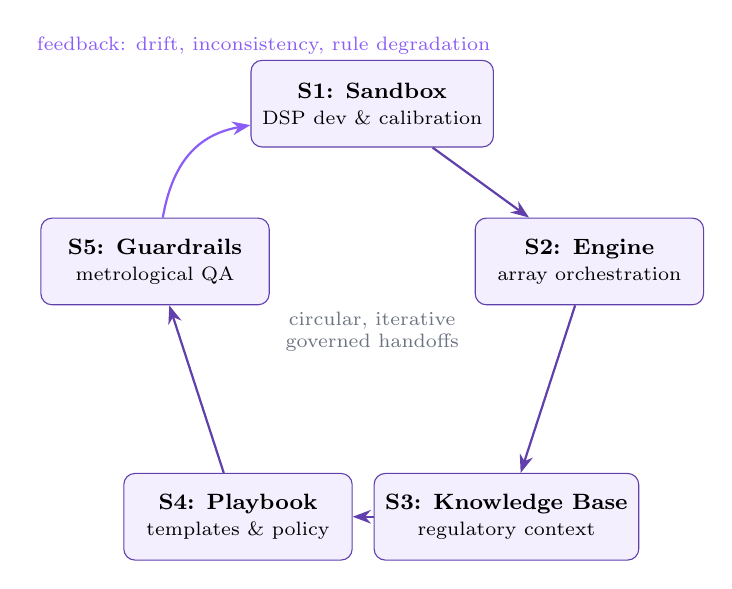
\begin{tikzpicture}[
  font=\footnotesize,
  >={Stealth[length=2.4mm]},
  stage/.style={draw=violet!70!black, fill=violet!10, rounded corners=4pt,
                align=center, minimum width=2.9cm, minimum height=1.1cm, inner sep=4pt},
  arr/.style={draw=violet!70!black, thick, -{Stealth}}
]
\node[stage] (s1) at (90:2.9)   {\textbf{S1: Sandbox}\\{\scriptsize DSP dev \& calibration}};
\node[stage] (s2) at (18:2.9)   {\textbf{S2: Engine}\\{\scriptsize array orchestration}};
\node[stage] (s3) at (-54:2.9)  {\textbf{S3: Knowledge Base}\\{\scriptsize regulatory context}};
\node[stage] (s4) at (-126:2.9) {\textbf{S4: Playbook}\\{\scriptsize templates \& policy}};
\node[stage] (s5) at (162:2.9)  {\textbf{S5: Guardrails}\\{\scriptsize metrological QA}};

% Let TikZ choose optimal border anchors for each edge
\draw[arr] (s1) -- (s2);
\draw[arr] (s2) -- (s3);
\draw[arr] (s3) -- (s4);
\draw[arr] (s4) -- (s5);
% Feedback loop: S5 back to S1, curved above
\draw[arr, violet] (s5) to[out=80, in=190, looseness=1.1] (s1);
\node[font=\scriptsize, text=violet, anchor=south] at ($(s5.north)!0.5!(s1.north)+(0,0.95)$)
  {feedback: drift, inconsistency, rule degradation};

\node[font=\scriptsize, text=vgrey, align=center] at (0,0)
 {circular, iterative\\governed handoffs};
\end{tikzpicture}
\caption{PCG (Layer~3): five circular stages. Stage~5 outputs feed Stage~1, closing the loop;
the numbered labels identify functional ownership, not a mandatory chronological order for
regulatory decision execution.}
\label{fig:pcg}
\end{figure}

\subsection{The five stages}
\label{sec:stages}

\begin{enumerate}
  \item \textbf{Stage 1 --- RF/DSP Development \& Calibration Sandbox (the Sandbox).} A safe,
    collaborative space for building and testing DSP algorithms, calibration procedures, and
    measurement pipelines before field deployment: signal-analysis notebooks (GNU Radio
    Companion, Python/SciPy) for rapid prototyping on captured I/Q; hardware-in-the-loop IDEs
    for production DSP code on embedded hosts; version control for block diagrams, calibration
    coefficients, and detection rules; containerization for reproducible environments across
    workstations and field targets. \emph{Output:} validated DSP blocks, calibrated measurement
    procedures, and feature prototypes, which enter Stage~2 as deployment candidates; Stage~1
    also receives Stage~5 drift reports, validation failures, and uncertainty anomalies as
    prioritized inputs for the next cycle.
  \item \textbf{Stage 2 --- Array Orchestration \& Multi-Node Coordination (the Engine).}
    Coordination of distributed SDR nodes, measurement workflows, and multi-node data fusion: an
    array orchestrator scheduling wideband acquisitions and cross-node campaigns; workflow
    orchestrators (GNU Radio, Apache Airflow, custom DSP schedulers); multi-node coordination
    roles (acquisition scheduler, calibration manager, timing supervisor, fusion arbiter); and
    data-routing gateways with local buffering during link outages. \emph{Output:} structured
    measurement decisions, capability-eligibility records, eligibility-gated decision records,
    synchronized observation epochs, and traceable chains from node-level results to array-level
    regulatory conclusions. Formal compliance decisions are produced only after the regulatory
    context and measurand-specific decision rule have been resolved and the applicable gate has
    been passed (\cref{sec:authority}).
  \item \textbf{Stage 3 --- Regulatory \& Spectral Knowledge Base (the Knowledge Base).}
    Authoritative regulatory context, licensed-station parameters, and historical spectral
    reference data grounding every measurement in validated information: regulatory and spectral
    data retrieval, where sources used for formal compliance carry an applicability record
    (jurisdiction, competent authority, service, station, effective date, source version,
    precedence rule); historical spectrum embeddings for trend comparison and anomaly
    fingerprinting; and knowledge graphs of station relationships, propagation characteristics,
    array topology, and inter-node calibration histories. \emph{Output:} contextual regulatory
    grounding and versioned measurand-specific decision definitions (rule type, limits or
    permitted region, reference quantities, rule parameters, regulatory source).
  \item \textbf{Stage 4 --- Measurement Configuration \& Policy Playbook (the Playbook).}
    Standardization and version control of measurement configurations, calibration profiles, and
    regulatory decision rules: measurement templates (parameterized channel plans, detection
    rules, spectral configurations); calibration-profile versioning (primary, secondary, and
    relative states, coefficients, validity periods across nodes); A/B testing of DSP variants
    against controlled reference signals with versioned acceptance criteria and rollback
    thresholds; and policy enforcement for gain limits, metadata formats, capability-eligibility
    requirements, and decision-rule integrity. \emph{Output:} consistent, governed, optimized
    measurement configurations deployable to the array with full traceability to regulatory rule
    sets and calibration states.
  \item \textbf{Stage 5 --- Metrological QA \& Array Health Guardrails (the Guardrails).}
    Measurement of RF and DSP performance, detection of metrological drift, validation of
    cross-node consistency, and enforcement of array-health boundaries: evaluation metrics
    (carrier-frequency error, calibrated power accuracy, occupied-bandwidth containment, false
    occupancy rate, missed detection rate, cross-node consistency score); human-in-the-loop
    review of anomalous regulatory classifications; observability (sample-loss events, I/Q
    residuals, DC contamination, timing skew, calibration validity, reference-lock state, drift,
    processing load, memory, ADC dynamic-range utilization); and alerting on threshold
    exceedances and health degradation. \emph{Output:} performance reports, calibration-drift
    logs, uncertainty scores, and health-state classifications, consumed by Stage~1 to initiate
    the next improvement cycle---closing the loop.
\end{enumerate}

The numbered stage labels identify \emph{functional ownership}, not a mandatory chronological
order. Governed handoffs bind the stages: Stage~1 outputs become deployment candidates for
Stage~2 under a versioned Stage~4 configuration; Stage~3 supplies regulatory grounding to Stage~4
before rules are activated; Stage~4 publishes the versioned template, calibration profile,
capability class, and decision configuration consumed by Stage~2; Stage~2 executes acquisitions,
eligibility gating, and (only for eligible measurands) the configured formal decision logic; and
Stage~5 evaluates performance, uncertainty, drift, and cross-node consistency, feeding Stage~1
while also constraining or downgrading Stage~4 configurations and Stage~2 execution.

\subsection{Production Promotion and Rollback Gate}
\label{sec:promotion}

This gate is the Layer~2/Layer~3 contract (\cref{sec:l2-l3}). A Stage~1 deployment candidate
shall not enter governed Stage~2 production execution until a versioned promotion record
confirms:

\begin{enumerate}[label=(\roman*)]
  \item the Stage~1 validation package and candidate identifier;
  \item the active Controlled Source Specification Baseline and Stage~3 regulatory-rule version;
  \item the Stage~4 measurement template, calibration profile, capability state, acceptance
    criteria, and rollback thresholds;
  \item a valid Stage~5 metrological and node-health state;
  \item approval by the deployment authority identified in the Stage~4 policy record.
\end{enumerate}

Initial activation uses the node subset or rollout scope authorized by that record. Stage~5 then
evaluates the configured post-deployment acceptance metrics over the defined evaluation interval.
Exceedance of a rollback threshold, loss of calibration validity, invalidation of the regulatory
baseline, or a safety/health gate failure suspends the candidate and restores the last approved
compatible configuration. Promotion, rejection, rollback, and restoration events are preserved as
versioned evidence records.

\subsection{Capability-class lifecycle}
\label{sec:capability}

Four capability classes---\textbf{Unsupported} $\rightarrow$ \textbf{Screening-Grade}
$\rightarrow$ \textbf{Conditional Compliance-Grade} $\rightarrow$
\textbf{Compliance-Grade}---each add a layer of validation obligation on top of the last rather
than forming a separate track. A new measurand or algorithm enters in Stage~1 as Unsupported or
Screening-Grade; Stage~3 resolves the applicable regulatory context; Stage~4 versions the
screening template and profile with formal compliance output disabled; after the Promotion Gate
confirms the authorized screening rollout, Stage~2 deploys to the approved node subset; Stage~5
accumulates the uncertainty, repeatability, consistency, and health evidence required by the
Capability Qualification Record. Promotion to Conditional Compliance-Grade requires approval of
that record; promotion to Compliance-Grade requires that all measurand-specific preconditions in
the Controlled Source Specification Baseline be implemented, independently validated, and
recorded. Each transition is controlled by a versioned record (measurand, current and proposed
states, required evidence, acceptance criteria, validation method, validator identity and
independence, approving authority, resulting configuration version), and the validation authority
must be independent of whoever produced the candidate evidence---the organizational expression of
the oracle-$\neq$-generator principle. Promotion and demotion events are themselves logged as
Stage~5 outputs feeding Stage~1.

\subsection{GUM uncertainty propagation}
\label{sec:gum}

The GUM uncertainty framework is embedded at each measurement-relevant stage boundary, and each
stage's contribution to (or exclusion from) the uncertainty budget is explicitly identified:

\begin{itemize}
  \item \textbf{Stage 1:} each uncertainty component is classified by its \emph{method of
    evaluation}, not by its physical source. \textbf{Type A} evaluation is used when the standard
    uncertainty comes from statistical analysis of measured quantity values; \textbf{Type B} when
    it comes from calibration certificates, specifications, prior data, or documented scientific
    judgment. Algorithmic, hardware, timing, and environmental effects may therefore contribute
    through either category according to the evidence used. The evaluation method, source data,
    statistical model, sensitivity coefficient, and resulting standard uncertainty are attached
    to the applicable DSP block or calibration coefficient.
  \item \textbf{Stage 2:} timing skew, sample-loss effects, and inter-node residual mismatch are
    quantified when they influence a reported measurand, classified Type A or Type B by
    evaluation method, and---including covariance terms where input quantities are
    correlated---propagated into the node-level uncertainty budget.
  \item \textbf{Stage 3:} the regulatory decision reference is represented by its governing
    mathematical form (one-sided limit, two-sided tolerance interval, permitted range,
    frequency-dependent limit or emission mask $T(f)$, relative reference, or temporal/occupancy
    criterion). These are authoritative \emph{decision inputs}, not measurement-error
    contributions to the budget; the source version, retrieval timestamp, decision-rule type, and
    active parameters are logged as configuration metadata so the rule applied to each
    determination can be reconstructed.
  \item \textbf{Stage 4:} measurement-template versioning captures which uncertainty
    contributions were active at the time of configuration deployment.
  \item \textbf{Stage 5:} the combined standard uncertainty $u_c(y)$ and expanded uncertainty $U$
    are validated from the aggregated contributions; drift detection compares current uncertainty
    envelopes against the calibration record. Stage~2 computes real-time measurement uncertainty
    using Stage~5-approved models, so Stage~1 receives not only \emph{what} degraded, but with
    \emph{what confidence} the degradation was detected.
\end{itemize}

Related to this, the Ground-Truth Reference Contract constrains how performance is measured at
all: false-occupancy and missed-detection rates used for Stage~5 acceptance or feedback are
computed only over observations carrying a qualified Ground-Truth Reference Record (reference
source and authority, labelled state, time/frequency bounds, alignment tolerances, review status,
dataset version). Ambiguous labels are excluded or reported separately as indeterminate, and
Stage~5 reports the numerator, denominator, reference identifiers, and excluded cases with every
result used to trigger a production change.

\subsection{Regulatory Decision Authority and dependency contract}
\label{sec:authority}

The circular architecture shall not be read as a temporal sequence in which Stage~2 may issue a
formal regulatory decision before Stages~3--5 have supplied the control information the framework
requires. For each measurand and decision cycle: Stage~3 provides the authoritative regulatory
context and measurand-specific decision definition; Stage~4 binds it to the deployed measurement
template, calibration profile, capability class, and versioned decision configuration; Stage~5
provides the current metrological-validity and health information; and only then does Stage~2
execute the measurement workflow, apply active Stage~4 calibration coefficients to raw I/Q, and
pass the measurand through the Capability Eligibility \& Regulatory-Use Gate before formal
decision logic. The rule itself must define how the measured value and its uncertainty enter
acceptance, rejection, and any indeterminate or guard-band outcome. Screening-grade results may
generate screening or review events but remain distinct from formal compliance determinations, and
unsupported measurands are blocked from regulatory decision processing entirely.

\subsection{The four feedback mechanisms}
\label{sec:feedback}

The loop closes through four primary mechanisms, all Stage~5$\rightarrow$Stage~1:

\begin{enumerate}
  \item \textbf{Calibration drift detection:} Stage~5 identifies frequency-reference offset or
    gain bias beyond Tier~2 limits $\rightarrow$ Stage~1 executes recalibration experiments
    $\rightarrow$ Stage~4 updates calibration-profile versions.
  \item \textbf{Cross-node inconsistency:} Stage~5 flags persistent disagreement beyond the
    uncertainty budget $\rightarrow$ Stage~1 investigates propagation-model or DSP-algorithm
    errors $\rightarrow$ Stage~3 updates the knowledge graph or station records.
  \item \textbf{Detection rule degradation:} Stage~5 evaluates false-occupancy and
    missed-detection rates against qualified ground-truth records $\rightarrow$ Stage~1 prototypes
    improved detection algorithms $\rightarrow$ Stage~4 evaluates the candidate against the
    Promotion Gate $\rightarrow$ Stage~2 deploys only an approved update to the authorized
    rollout scope.
  \item \textbf{Resource optimization:} Stage~5 analyses ADC dynamic-range utilization and
    processing load $\rightarrow$ Stage~1 prototypes efficient DSP implementations
    $\rightarrow$ Stage~4 simplifies measurement configurations.
\end{enumerate}

Health-driven degradation is the guardrail counterpart: a node flagged \emph{operational for
screening only} has its Stage~4 templates automatically downgraded and is excluded from compliance
fusion; a \emph{degraded} node is suspended from fusion and locked pending Stage~1 investigation;
an \emph{unavailable} node is removed from the orchestration schedule while Stage~5 continues to
log absence events.

\subsection{Audit-ready evidence archiving}
\label{sec:archiving}

Every completed loop through the five stages produces a controlled evidence record. For formal
compliance determinations the repository provides append-only or write-once protection,
authenticated access control, a cryptographic content digest for each retained artefact, an
integrity-protected manifest, a trusted acquisition timestamp, and a retention identifier;
corrections create a new linked record without overwriting the preserved predecessor. The record
covers acquisition metadata (centre frequency, sample rate, gain state, timestamp reference); the
DSP pipeline version, sandbox commit, container-image digest, and dependency manifest needed to
reproduce the executed DSP path; the orchestration log and node-eligibility list; the regulatory
rule set version and baseline identifier; the measurement-configuration version, calibration
profiles, capability state, and policy checks; estimated measurands, uncertainty budgets, decision
outcomes, health states, fusion weights, and ground-truth identifiers; and, for each formal
decision, the raw I\/Q interval---or another lossless source artefact that documented replay
validation has demonstrated sufficient to recompute every reported measurand. Reconstructability
is demonstrated by replay or equivalent deterministic verification for each production DSP release
before that release is authorized for formal compliance use. This is the Layer~1 evidence
discipline, industrialized: the same principle (recorded measurements, pre-declared criteria,
reproducible execution) now applies to every production decision.

% ===========================================================================
\section{Inter-Layer Integration}
\label{sec:integration}

The three layers compose because each layer's terminal output is the next layer's input. This
section states both couplings and the artefact-to-stage mapping that implements them.

\subsection{Layer 1 $\rightarrow$ Layer 2}
\label{sec:l1-l2}

The \textbf{Ctx 03 Build Package} becomes the executable specification for CI+SIL: component
contracts, schemas, error behaviour, and the declared unit/integration/acceptance tests are
exactly what the pipeline executes. \textbf{Artefact~3} (eval and benchmarking suites) seeds the
CI regression baseline---the suites zz\_Workflow already requires \emph{are} the CI harness, so
the coupling adds automation and not concepts. Three artefacts complete the interface: the Ctx 01
measurable acceptance criteria become the deterministic gate's thresholds; Artefact~4's guardrail
rules become expected behaviours in the suite (e.g.\ the ``Uncertain''-below-threshold rule must
be tested); and Artefact~5's telemetry continues uninterrupted into CI, where failure classes
route via R0--R3 to the Ctx stage that must revise. The name of the handoff output stays honest:
Layer~2 terminates in a \emph{regression-passing build}, which is \verified, not \validated.

\subsection{Layer 2 $\rightarrow$ Layer 3}
\label{sec:l2-l3}

The coupling is the \textbf{Production Promotion and Rollback Gate} (\cref{sec:promotion}), a
versioned contract with five prerequisites that bind the CI world to the operations world: the
Stage~1 validation package (fed by Layer~2 evidence); the Stage~3 regulatory baseline; the Stage~4
measurement template and calibration profile; the Stage~5 metrological-validity state; and human
approval by the deployment authority. In the other direction, Stage~5 feedback re-enters Layer~2
as ordinary CI triggers: a calibration-coefficient change is a code change, a regulatory-rule
update is a context change, and a model or prompt change in any LLM-assisted component fires the
full suite---the four trigger classes of \cref{sec:triggers} apply unchanged in production.

\subsection{Artefact-to-stage mapping}
\label{sec:mapping}

\cref{tab:mapping} maps each zz\_Workflow governing artefact to the PCG stage it feeds. The
mapping is one-to-many for the artefacts that carry governance (3 and 6), and it shows that no
artefact dies at the layer boundary: everything Layer~1 defines, Layer~3 operationalizes.

\begin{table}[htbp]
\centering
\caption{Which Layer~1 artefact feeds which Layer~3 stage.}
\label{tab:mapping}
\small
\begin{tabular}{@{}lp{9.6cm}@{}}
\toprule
\textbf{Layer~1 artefact} & \textbf{Feeds PCG stage(s)} \\
\midrule
1. System \& Prompt Architecture Map & Stage~2 orchestration logic (roles, routing, fallbacks) \\
2. Context \& Retrieval Specs & Stage~3 knowledge base (indexing, grounding, applicability records) \\
3. Eval \& Benchmarking Suites & Stage~1 sandbox validation; Stage~5 acceptance metrics against ground truth \\
4. Safety \& Guardrail Design Rules & Stage~5 guardrails (thresholds, ``Uncertain'' behaviour, HITL escalation) \\
5. AI Feedback \& Telemetry Specs & Stage~5 observability (failure classes, drift logs, anomaly records) \\
6. Data Privacy, Governance \& Compliance Specs & All stages (what may leave the environment, retention, redaction) \\
\bottomrule
\end{tabular}
\end{table}

\subsection{Extended defect routing}
\label{sec:extended}

Layer~1 routes a failed verification to the responsible Ctx stage (R0--R3). Layer~3 has an
analogous but circular mechanism: Stage~5 findings return to Stage~1 as prioritized validation
or refactoring targets. The two are structurally identical---a failure is classified by root
cause and sent to the stage that owns that cause---but differ in what ``the stage'' means. In
Layer~1 the stages are \emph{definition stages} (problem, requirements, design, contract); in
Layer~3 they are \emph{operational functions} (sandbox, engine, knowledge base, playbook,
guardrails). The R0 analogue in operations is the invalidation of the regulatory baseline, which
suspends the pipeline and forces a documented dependency-impact analysis before reactivation.

% ===========================================================================
\section{HITL and HIL Governance}
\label{sec:governance}

V-SIL's governance rests on two distinct human-and-hardware barriers, and conflating them is the
most common way a verification pipeline overstates its claims \cite{opalrt2026,sheridan2026b}.

\textbf{HITL is an authorization barrier.} A person approves consequential actions. In Layer~1
this is every gate: the two readiness gates H, the scope freeze, and the final acceptance
decision. In Layer~2 it is the human review of routed defects and of any change to the criteria
themselves. In Layer~3 it is the deployment-authority approval in the Promotion Gate, the
human-in-the-loop review of anomalous regulatory classifications in Stage~5, and the
independence requirement on the validating authority in each Capability Qualification Record.
Authorization is a decision about \emph{permission}; it is made by a person, on recorded
artefacts, and it is itself archived.

\textbf{HIL is a validation barrier.} The control software is exercised against real hardware:
acceptance testing at the apex of the V (\cref{fig:vsil}), where the Mock HAL is swapped for the
real device behind the same interface. HIL is the boundary of V-SIL's claims. Below the apex, the
system is \verified{} against pre-declared criteria on synthetic or replayed I/Q; only at the
apex---and ultimately in the field---does it become \validated{} \cite{sheridan2026b}. Simulation
has a ceiling, and HIL enters precisely when the restriction is hardware \cite{opalrt2026};
reported experience with LLM-assisted engineering shows that humans detect idealizations and
inconsistencies that automated evaluation misses entirely \cite{heinrichs2026,bajestani2026}.

\textbf{LLM governance rules.} Four rules bind model use across all three layers:

\begin{enumerate}[label=\textbf{G\arabic*.}]
  \item \textbf{The model never approves its own work.} Every gate in V-SIL is human-decided,
    and every acceptance decision is made by an external oracle.
  \item \textbf{Mechanical rejection beats LLM approval, never the reverse.} Schema violations,
    failed tests, and threshold exceedances reject work mechanically
    \cite{mcp2025,tooluse2026}; a model's approval cannot override a mechanical rejection, but a
    human may escalate one.
  \item \textbf{Acceptance by pre-declared criteria on recorded measurements, never by model
    judgement.} This is stated verbatim in Layer~1 and enforced by the deterministic gate of
    Layer~2 and the Promotion Gate of Layer~3.
  \item \textbf{Self-reported correctness is weak evidence.} Benchmarks that score accuracy alone
    reward confident guessing, so models are trained to hallucinate \cite{kalai2026}; where an
    LLM judge is used, it is calibrated against human raters with $\kappa \geq 0.6$ and bias
    controls \cite{futureagi2026,judge2026}, and it never gates acceptance.
\end{enumerate}

The LLM's legitimate roles are drafting, translation between artefacts, anomaly triage, and
telemetry summarization---all upstream of a gate, none at a gate. Two-level control operationalizes
this: the model plans at the slow level; a deterministic controller executes the fast loop; the
model never sits inside a real-time loop, and physical limits declared in a tool's JSON schema are
the first line of defence, since a call violating the schema is rejected before it reaches the
device \cite{tooluse2026,mcp2025}. Where autonomous chains are used, their length is bounded:
reliability decays roughly geometrically with sequential steps, with a practical ceiling near 16
\cite{mittal2026}, which is why every stage in V-SIL is short, bounded, and human-gated.

% ===========================================================================
\section{Gaps and Maturity Assessment}
\label{sec:gaps}

Honesty about maturity is part of the method. \cref{tab:gaps} lists the components V-SIL depends
on that are not yet implemented or instantiated, with the gap each one leaves.

\begin{table}[htbp]
\centering
\caption{Maturity assessment: explicit gaps.}
\label{tab:gaps}
\small
\begin{tabular}{@{}lp{3.1cm}p{7.2cm}@{}}
\toprule
\textbf{Component} & \textbf{Status} & \textbf{Gap} \\
\midrule
HIL bench & Not implemented & No live-RF validation infrastructure; the apex of the V cannot yet be exercised, so all claims remain at the SIL level of verification \\
MCDA \cite{mcda2026} & Not implemented & Multi-hypothesis selection (Ctx 02 trade study) is not formalized into a repeatable decision procedure \\
Controlled Source Specification Baseline & Not instantiated & Stage~2 formal compliance execution remains disabled until the Stage~4 baseline record is populated and approved \\
Single-to-array scaling & Not covered & The pipeline assumes a sensor array, but no methodology exists for scaling the Layer~1/2 single-node results to array level \\
LLM governance in production & Not specified & Use constraints for LLMs inside Stage~2 (orchestration) and Stage~5 (review support) are undefined \\
\bottomrule
\end{tabular}
\end{table}

None of these gaps is structural. The HIL bench is an infrastructure project that the Mock HAL
already anticipates through its same-interface swap; MCDA formalizes a trade study that Ctx 02
already performs informally; the Controlled Source Specification Baseline is a document-binding
task with a defined record schema; single-to-array scaling is a research programme rather than a
methodology gap; and production LLM governance can be written as an extension of the four rules
in \cref{sec:governance}, constrained by the same gates.

% ===========================================================================
\section{Conclusion}
\label{sec:conclusion}

V-SIL unifies three bodies of methodology---conceptual validation (zz\_Workflow), continuous
software development (CI+SIL), and post-development operations (PCG)---into a single governed
lifecycle for LLM-assisted SDR FM spectrum-sensing systems. Each layer has a distinct role:
Layer~1 \emph{defines} what to build and validates the concept and design; Layer~2
\emph{implements} it and verifies it continuously; Layer~3 \emph{operates} the deployed system
under metrological and regulatory governance.

The coupling is clean because each layer's terminal output is the next layer's input: the Ctx 03
Build Package is Layer~2's executable specification; Artefact~3 is already the CI regression
harness; and the Promotion Gate binds the regression-passing build to the production pipeline as
a versioned, revocable contract. Nothing is invented at the boundaries, which is why the
methodology can be adopted incrementally.

The claims stay honest by construction. The system is \verified{} at software-in-the-loop and
\validated{} only at hardware-in-the-loop and in the field; every claim names the environment in
which its evidence was produced. The model drafts but never approves: mechanical rejection beats
LLM approval, never the reverse, and acceptance is decided by pre-declared criteria applied to
recorded measurements. Five gaps remain---a HIL bench, formalized MCDA, an instantiated Controlled
Source Specification Baseline, a single-to-array scaling methodology, and production LLM
governance---and each is explicit, bounded, and tractable.

% ===========================================================================
\appendix
\section*{References}
\label{sec:references}
\addcontentsline{toc}{section}{References}

\begin{thebibliography}{99}\small
\bibitem{tooluse2026} Harbin Institute of Technology \& Harvard, ``The Evolution of Tool Use in LLM Agents,'' arXiv:2603.22862, Mar.\ 2026.
\bibitem{kalai2026} A.\ T.\ Kalai \emph{et al.}, ``Evaluating LLMs for accuracy incentivizes hallucinations,'' \emph{Nature}, vol.\ 653, Apr.\ 2026.
\bibitem{mittal2026} Mittal, ``How Fast Do Agents Rot?,'' arXiv:2609.01660, Sep.\ 2026.
\bibitem{anthropic2026} Anthropic, ``Effective context engineering for AI agents,'' 2026.
\bibitem{nerd2026} Nerd Level Tech, ``AI Agent Reliability 2026: Structure Beats Instructions,'' 2026.
\bibitem{mcp2025} Model Context Protocol Specification, rev.\ 2025-06-18, \url{modelcontextprotocol.io}.
\bibitem{opalrt2026} OPAL-RT, ``Guide to HIL Testing,'' updated Sep.\ 2026.
\bibitem{verifgap2026} ``Autonomous Research Agents: Verification Gap,'' arXiv:2608.05179, Jun.\ 2026.
\bibitem{judge2026} ``LLM-as-a-Judge Is Not an Oracle,'' arXiv:2609.02246, Sep.\ 2026.
\bibitem{qmsdoc2026} QMSdoc, ``Traceability in V-Model,'' Jan.\ 2026.
\bibitem{sheridan2026a} Sheridan, ``Testing Embedded Systems 2026,'' Apr.\ 2026.
\bibitem{heinrichs2026} Heinrichs \emph{et al.}, ``From Prompt to Prototype: LLM-Driven RF Workflow,'' arXiv:2608.31006, Aug.\ 2026.
\bibitem{bajestani2026} Sadeqi Bajestani \emph{et al.}, ``HITL+LLM in smart manufacturing,'' \emph{J.\ Manufacturing Systems}, vol.\ 86, Jun.\ 2026.
\bibitem{futureagi2026} FutureAGI, ``LLM-as-a-Judge in 2026,'' updated Aug.\ 2026.
\bibitem{mcda2026} \emph{Sustainable Futures}, ``MCDA reliability,'' Jun.\ 2026.
\bibitem{sheridan2026b} Sheridan Tech, ``Design Validation vs Verification,'' Mar.\ 2026.
\bibitem{pith2026} Pith, ``Introducing Background Temperature,'' arXiv:2604.22411, 2026.
\end{thebibliography}

\end{document}
